\documentclass[11pt,a4paper]{article}

% ---------------------------------------------------------------------------
% Packages
% ---------------------------------------------------------------------------
\usepackage[utf8]{inputenc}
\usepackage[T1]{fontenc}
\usepackage[british]{babel}
\usepackage{microtype}
\usepackage[a4paper,margin=2.6cm]{geometry}
\usepackage{amsmath,amssymb}
\usepackage[authoryear,round]{natbib}
% This paper's bibliography is hand-written (no BibTeX/.bbl), with multi-author \bibitem optional
% labels (e.g. "Smith, Jones and Lee, 2020") that natbib's own BibTeX-standard-compatibility
% self-check does not expect; that check is purely an internal sanity test run at \end{document}
% and does not affect how \citep/\citet actually render (both already read the \bibitem labels
% directly), so it is neutralized here rather than reformatting 160 manually-written entries.
\makeatletter
\let\NAT@force@numbers\relax
\makeatother
\usepackage{booktabs}
\usepackage{longtable}
\usepackage{array}
\usepackage{graphicx}
\usepackage{caption}
\usepackage{enumitem}
\usepackage{xcolor}
\usepackage[colorlinks=true,linkcolor=blue!50!black,citecolor=blue!50!black,urlcolor=blue!50!black,bookmarksnumbered=true]{hyperref}
\usepackage{fancyhdr}
\usepackage{setspace}
\usepackage{titlesec}
\usepackage{abstract}

\renewcommand{\abstractnamefont}{\normalfont\bfseries}
\renewcommand{\abstracttextfont}{\normalfont\itshape}

\titleformat{\section}{\normalfont\large\bfseries}{\thesection}{1em}{}
\titleformat{\subsection}{\normalfont\bfseries}{\thesubsection}{1em}{}

\pagestyle{fancy}
\fancyhf{}
\fancyhead[L]{\small\textit{A stochastic scenario model of state size and fiscal reform in Brazil}}
\fancyhead[R]{\small\thepage}
\renewcommand{\headrulewidth}{0.3pt}

\setstretch{1.04}

\newcommand{\pp}{\,pp}
\newcolumntype{R}[1]{>{\raggedleft\arraybackslash}p{#1}}

\title{\textbf{Reducing, Holding and Expanding the Size of the State: \\
A Modular Stochastic Framework for Evaluating Fiscal Reform Scenarios in Brazil, with an Application to the 2026 Presidential Programmes}}

\author{Flaviano A.\ Moreira\thanks{Independent research; no institutional affiliation. Correspondence: \texttt{flaviano.a.moreira@gmail.com}. ORCID: \href{https://orcid.org/0009-0009-0783-5477}{0009-0009-0783-5477}. Data and code availability, funding, conflict of interest, ethics, author contribution (CRediT) and AI-tool disclosure statements appear before the references.}}

\date{\today}

\begin{document}

\maketitle

\begin{abstract}
\noindent This paper builds a modular, stochastic simulation framework for Brazilian fiscal policy, chaining macroeconomic, microsimulation, social, feedback, external and governance blocks into a thousand-draw Monte Carlo reporting paired scenario differences over five- to twenty-year horizons, and applies the same machinery to the two 2026 presidential candidates' filed fiscal programmes. A historical back-test shows the model tracks year-on-year fiscal changes within a stated tolerance, but its seven-year-ahead debt-level reconstruction overshoots observed 2024 debt by 12--16 percentage points of GDP, a failure traced to discretionary balance-sheet operations, not a mis-specified equation; we widen uncertainty bands with a stochastic adjustment term rather than fit a correction to noise, and publish only paired differences, never a validated debt level. A set of off-by-default diagnostics on the business cycle, monetary policy, the exchange rate and interest-income incidence shows one channel reverses the paper's headline distributional finding once interest income is allocated as it is actually held, and understates a debt-financed expansion's true debt cost by 13--14\%. The framework's contribution is a disciplined, fully traceable accounting of what a stated fiscal composition and size imply.
\end{abstract}

\noindent\textbf{Keywords:} fiscal consolidation; debt sustainability; Monte Carlo microsimulation; state size; Brazil; corruption and governance; fiscal multipliers.

\noindent\textbf{JEL classification:} H62 (deficit; surplus); H63 (debt; debt management); H50 (national government expenditures and related policies); C63 (computational techniques; simulation modelling); I38 (government policy; welfare and poverty programmes); D31 (personal income, wealth and their distributions).

\vspace{0.3cm}

% ===========================================================================
\section{Introduction}
% ===========================================================================

A perennial question in the political economy of public finance is how much the state should tax and spend, and how the answer changes an economy's growth, its public debt, and the distribution of income and health across its population. Brazil poses this question with unusual sharpness. General-government primary spending reached 39.8\% of GDP in 2025, population ageing is projected to raise the age-related share of that spending by a further 3.3 percentage points of GDP (pp GDP) over the subsequent decade even with no policy change \citep{ibge2024,tesouro2025}, and gross general-government debt stood at 78.6\% of GDP at the close of 2025 \citep{bcbsgs}. The 2026 presidential run-off has, in turn, placed two sharply different fiscal philosophies before voters: a constitutional spending-growth rule tying real federal expenditure growth to a fraction of real revenue growth, and a debt-stabilising primary-balance rule that moves the government's balance linearly towards the level implied by the debt dynamics identity.

This paper documents a model built to make that debate tractable without pretending to resolve it. We did not set out to forecast Brazil's fiscal future, nor to rank the candidates. We set out to build an instrument that takes a stated change in the size and composition of the state --- expressed, deliberately, in the same units a finance ministry would use, percentage points of GDP --- and propagates it consistently through growth, debt, household incomes, health outcomes, long-run human- and physical-capital accumulation, the external sector, and an explicit account of leakage and corruption risk, while reporting at every step how much of the result is a sourced estimate, a defensible modelling choice, or an acknowledged gap. Every numerical parameter in the model is traceable to a single registry file with its source, vintage and licence; where no credible estimate exists the model raises an error rather than silently substituting a plausible number. This discipline is, we think, the paper's main methodological claim: a scenario model's usefulness depends less on the sophistication of any one equation than on the auditability of the whole chain and the honesty with which it reports its own failures.

The remainder of the paper proceeds as follows. Section~\ref{sec:lit} places the model within eleven strands of literature, from the broad composition-of-consolidation and fiscal-multiplier debates through stochastic debt-sustainability analysis, debt-threshold and interest-growth-differential dynamics, the distributional and social consequences of adjustment, microsimulation and fiscal-incidence methodology, sovereign risk premia and fiscal fatigue, governance and corruption, fiscal-rule design, and the stock-flow-adjustment literature that turns out to anticipate this paper's own central finding. Section~\ref{sec:context} sketches the Brazilian fiscal and demographic context the model takes as given. Section~\ref{sec:architecture} describes the modular architecture and the nine chained blocks. Section~\ref{sec:scenarios} defines the baseline, reduction and expansion scenarios and explains how the two 2026 candidate programmes are mapped onto the same machinery. Section~\ref{sec:montecarlo} describes the Monte Carlo design and the uncertainty it does and does not capture. Section~\ref{sec:backtest} reports the model's historical back-test honestly, including the dimension on which it fails, and summarises the diagnostic extensions, given in full in the online supplementary material, built in direct response to that failure. Section~\ref{sec:results} summarises the headline, gate-cleared results. Section~\ref{sec:discussion} discusses limitations and the appropriate use of the model, and Section~\ref{sec:conclusion} concludes.

To anchor what follows in numbers before the mechanics behind them are introduced: under the model's own status-quo baseline, debt/GDP rises from 78.6\% in 2025 to a central 145.5\% by 2035, driven mainly by the interest-growth differential rather than discretionary policy (Section~\ref{sec:results}); against that baseline, a central, sustained 4~pp-of-GDP consolidation lowers ten-year debt by a little under 24~pp of GDP at a median GDP cost of under one percentage point under transitory multipliers; and the model's own historical back-test fails at the level of absolute debt, though not at the level of paired scenario differences (Section~\ref{sec:backtest}), which is why every comparison in this paper is reported as a difference against the baseline, never as a validated level. A later diagnostic (reported in full in the online supplementary material; Section~\ref{sec:discussion}) finds that one of the paper's own headline distributional results reverses sign once a channel the published Monte Carlo does not model is added --- a finding we report in full rather than soften, for the same reason we report the back-test failure in full.

% ===========================================================================
\section{Related literature}
\label{sec:lit}
% ===========================================================================

Across these eleven strands, one gap recurs: existing debt-sustainability, multiplier and distributional literatures are each well developed on their own, but rarely chained into a single, auditable instrument that propagates one stated policy change through growth, debt, household incomes and social outcomes together, and checks the result against the country's own history before reporting it. That gap is what this paper tries to fill. This section positions the model against the eleven strands; the online supplementary material gives the full discussion, with every supporting citation, theme by theme. The summary here keeps only the most load-bearing references in each strand.

On the \emph{composition of fiscal consolidation}, \citet{alesinaardagna2010,alesinafaverogiavazzi2015} find spending-based adjustment plans produce milder output losses than tax-based ones, a finding \citet{guajardoleighpescatori2014} contest using narrative identification that rejects ``expansionary austerity'' more broadly. We take no position: the model reports whatever composition the user specifies, using Brazil-specific rather than imported multipliers. On \emph{multiplier size and state-dependence}, \citet{auerbachgorodnichenko2012} and \citet{ilzetzkimendozavegh2013} are the central references, the latter showing multipliers fall with debt, trade openness and exchange-rate flexibility in ways that place an economy such as Brazil's towards the lower end of the range; \citet{pires2014} and \citet{resendepires2021} provide the Brazil-specific estimates this model's category-specific multipliers are checked against.

On \emph{stochastic debt-sustainability analysis}, the model's direct methodological ancestor is \citet{celasundebrunostry2007}'s fan-chart approach, which \citet{garciarigobon2004} and \citet{karamhostland2005,karamhostland2006} apply to Brazilian and emerging-market debt specifically; \citet{levyyeyatisturzenegger2023} offer a more recent balance-sheet reformulation of the same question, and \citet{prasadetal2019growthatrisk,lianpresbiterowiriadinata2020} point towards the conditional-quantile ``debt-at-risk'' framing that a resampled Monte Carlo such as this one approximates but does not formally implement (a limitation Section~\ref{sec:discussion} returns to). On \emph{debt thresholds and the interest-growth differential}, \citet{reinhartrogoff2010} and its correction by \citet{herndonashpollin2014} are the cautionary precedent against single-threshold summaries, reinforced by \citet{egert2015} and \citet{panizzapresbitero2014}; \citet{blanchard2019}'s finding that $r<g$ has historically been closer to the norm than the exception directly motivates the paper's own result that the interest-growth differential, not the primary balance, dominates Brazil's projected debt path.

On the \emph{distributional and social consequences of adjustment}, \citet{ballfurcerilleighlloungani2013,woobovakindazhang2017} establish that consolidation raises the Gini coefficient, more so when spending-based; \citet{lagopenasetal2024} add a political-economy dimension, showing voters' tolerance for austerity depends on its financing instrument and their own ideology. \citet{szkloclarkerocha2024} and \citet{rasellaetal2013} are the Brazilian evidence behind the health-spending and cash-transfer channels respectively, read against \citet{filmerpritchett1999}'s scepticism that cross-country health spending alone explains mortality. On \emph{microsimulation methodology}, \citet{bourguignonspadaro2006} sets out the comparative-statics case this paper's own household block follows; \citet{higginspereira2014} apply the Commitment to Equity framework to Brazil directly, and \citet{balladaresgarciamiralles2026} is a recent demonstration, in this journal, of exactly this style of tax-record microsimulation applied to a live policy question.

On \emph{sovereign risk premia and fiscal fatigue}, \citet{baldaccikumar2010} anchors this model's linear premium coefficient, while \citet{ghoshkimmendozaostryqureshi2013} and \citet{bi2012} provide the nonlinear, fiscal-fatigue theory behind the diagnostic premium variant reported in the online supplementary material. On \emph{governance and corruption}, \citet{ferrazfinanmoreira2012,avisferrazfinan2018} supply the Brazilian audit evidence calibrating this model's leakage share; \citet{mauro1995,olken2007} are the foundational cross-country references, and \citet{hanousekkocenda2011} link corruption directly to fiscal performance, debt and deficits, across the new EU member states, a finding structurally close to this paper's own governance layer. On \emph{fiscal rules and the political economy of debt}, \citet{kopitssymansky1998} provide the taxonomy within which this paper situates the two 2026 candidate programmes as, respectively, an expenditure rule and a balance rule, without ranking them; \citet{feldkirchgassner2008} and \citet{lopezvillavicencio2025} are the closest real-world comparators.

Finally, and most consequentially for this paper's own validation result, the \emph{stock-flow-adjustment} literature independently documents exactly the phenomenon behind this model's Tier~2 back-test failure (Section~\ref{sec:backtest}): \citet{weber2012sfa} and \citet{jaramilloetal2017} show such adjustments are a large, persistent, poorly-explained source of debt accumulation worldwide, and that large adjustments predict debt subsequently failing to decline, while \citet{mackenziestella1996} explains why they occur at all (quasi-fiscal operations of public financial institutions, a description that fits BNDES's role in Brazil's own episode directly). \citet{gobettiorair2017} is the closest peer-reviewed reconstruction of the Brazilian episode specifically. The online supplementary material discusses all eleven strands, and every citation above, at full length.

% ===========================================================================
\section{Fiscal and demographic context}
\label{sec:context}
% ===========================================================================

Brazilian general-government primary spending was 39.76\% of GDP in the four quarters to 2025, against primary revenue of 38.97\% of GDP on the same General Finance Statistics Manual 2014 (GFSM) basis, implying a primary deficit of 0.79\% of GDP \citep{tesouro2025}. Gross general-government debt stood at 78.64\% of GDP in December 2025 \citep{bcbsgs}. Of primary spending, old-age and survivors' pensions (RGPS and, by proxy, RPPS) accounted for 11.65\% of GDP, health for 5.03\% and education for 5.10\%, using the 2024 COFOG functional classification carried forward one year \citep{tesourocofog2024}. Brazil's population is ageing: using National Transfer Accounts age-profiles for 2003 and 2018 \citep{nta2018} combined with the IBGE 2024 population revision \citep{ibge2024}, age-related spending alone is projected to rise by 3.3~pp of GDP over ten years and 7.3~pp over twenty, relative to a constant-spending-share counterfactual, with no change in policy or generosity.

This is the backdrop against which the 2026 presidential run-off programmes are written. The incumbent's programme is built around the existing constitutional spending-growth rule introduced by Complementary Law 200/2023 (``arcabou\c{c}o fiscal''), which ties real federal primary-spending growth to 70\% of real revenue growth, bounded between 0.6\% and 2.5\% a year. The challenger's programme proposes an explicit debt-stabilising primary-balance target, moving the federal government's primary balance over an unspecified number of years towards the level that would stabilise, rather than reduce, the debt ratio at its then-current level, financed partly through privatisation of state-owned enterprises. Section~\ref{sec:scenarios} explains how the model turns each rule into a comparable annual fiscal path without altering a single underlying equation.

% ===========================================================================
\section{Model architecture}
\label{sec:architecture}
% ===========================================================================

The model is organised as nine chained blocks, each with a narrow, tested public interface, so that later blocks consume only the outputs --- never the internal state --- of earlier ones. Every coefficient, elasticity, stock and share used anywhere in the chain is declared once, with its source, vintage and a verification flag, in a single parameter registry; a missing or unverifiable input raises an explicit error rather than being silently defaulted. Figure~\ref{fig:chain} sketches the dependency structure; we describe each block in turn.

\begin{figure}[htbp]
\centering
\footnotesize
\begin{tabular}{@{}l@{}}
Demographics (population, 2000--2070) $\longrightarrow$ Fiscal baseline (age-profile spending, \textsc{C1}) \\
\hspace{3.0cm}$\longrightarrow$ Macro block: growth, debt, revenue (\textsc{C2}) \\
\hspace{6.0cm}$\longrightarrow$ Household microsimulation (\textsc{C3}) \\
\hspace{6.0cm}$\longrightarrow$ Social outcomes: mortality, life expectancy (\textsc{C4}) \\
\hspace{6.0cm}$\longrightarrow$ Long-run feedback: schooling, health, capital, risk premium (\textsc{C5}) \\
\hspace{6.0cm}$\longrightarrow$ External block: terms of trade, FX (\textsc{C6}/\textsc{C7}) \\
\hspace{3.0cm}$\longrightarrow$ Governance: leakage (\textsc{G1}), major-corruption shocks (\textsc{G2}) \\
\hspace{3.0cm}$\longrightarrow$ Monte Carlo propagation (\textsc{D1}) $\longrightarrow$ Historical back-test (\textsc{D2}) \\
\hspace{0.3cm}$\dashrightarrow$ Online supplementary diagnostics: breach probabilities, FRF, nonlinear premium
\end{tabular}
\caption{The model's chained block structure. Each solid arrow is a one-directional, tested data interface; no downstream block mutates an upstream one. The dashed arrow marks the online supplementary diagnostics, which branch off the back-test gate, run only against \textsc{S0}, and never feed back into the scenario chain above.}
\label{fig:chain}
\end{figure}

\subsection{Demographic and age-profile fiscal baseline}

The baseline block projects Brazilian general-government primary spending under two polar rules: a status-quo rule (\textsc{S0}) in which pension and health spending drift with the population's age structure while every other category is held at its 2025 share of GDP, and a constant-size rule (\textsc{S1}) in which total primary spending is held at today's share of GDP, so that ageing-driven cost growth in pensions and health must be offset elsewhere. Age-specific per-capita transfer profiles for education, health and old-age/survivors pensions come from Brazilian National Transfer Accounts for 2003 and 2018 \citep{nta2018}; because the two vintages straddle the 2019 pension reform, the model evaluates both, together with three indexation rules (pure per-capita cost growth, pure GDP-per-working-age-person growth, and an equal-weighted blend), and reports the minimum and maximum of six resulting combinations as low/high bounds, with the 2018 profile at equal weight as the central case. The resulting \textsc{S0}--\textsc{S1} drift is 1.6/3.3/5.2/7.3~pp of GDP at five/ten/fifteen/twenty years (central estimates).

\subsection{Macroeconomic block: growth, debt and revenue}

The macro block converts an annual primary-spending path into output, debt and employment paths using a Cobb--Douglas production function,
\begin{equation}
Y_t = A_t K_t^{\alpha} (h_t L_t)^{1-\alpha},
\end{equation}
with capital accumulated endogenously, $K_t = (1-\delta)K_{t-1} + i_{t-1}Y_{t-1}$, rather than assumed to grow at a fixed rate. Capital share $\alpha$, depreciation $\delta$, the initial capital--output ratio and the investment rate are taken from Penn World Table 10.01 Brazil observations at constant 2017 prices \citep{pwt1001}; total factor productivity and human-capital growth are drawn from three overlapping sub-period compound annual growth rates (2000--2019, 2004--2013 and 2010--2019) to produce low/central/high bounds, since no single historical window is obviously the right one to extrapolate. Labour is population aged 15--64 at a fixed employment rate calibrated to its 2019 value; this omits any projected change in labour-force participation or the unemployment rate beyond an Okun-coefficient adjustment for demand-driven deviations.

Fiscal reductions or expansions below or above the \textsc{S0} path are translated into output effects through Brazil-specific accumulated fiscal multipliers by spending category --- public investment, social benefits, subsidies, and other current spending --- drawn from \citet{sanches2026} --- at the time of writing a working paper under review at \textit{Estudos Econ\^omicos} rather than yet formally published, a status we flag given how much of this block's calibration rests on it --- and reported as both a transitory impulse-response and a persistent, permanently-lower-output variant, since the wider multiplier literature (surveyed in the online supplementary material) does not agree on which horizon is appropriate --- \citet{auerbachgorodnichenko2012} and \citet{rameyzubairy2018} reach materially different conclusions on state-dependence even within a single, advanced-economy sample --- and the two horizons differ by an order of magnitude in their twenty-year debt consequences. Public debt accumulates through the standard identity
\begin{equation}
d_t = \frac{1+i_t}{1+g_t}\,d_{t-1} - pb_t + a_t,
\end{equation}
where $d_t$ is the debt-to-GDP ratio, $i_t$ the effective nominal interest rate, $g_t$ nominal GDP growth, $pb_t$ the primary balance and $a_t$ a residual debt adjustment (used, for instance, for privatisation proceeds or the stock-flow-adjustment noise term of Section~\ref{sec:backtest}). The effective real interest rate is estimated from the Fisher relation applied to five years (2021--2025) of observed interest payable over end-year gross debt and the contemporaneous GDP deflator, giving a historical range of $-2.04\%$ to $7.20\%$ and a median of $5.05\%$, reinflated at each projection corner by the corner's own deflator assumption.

With no policy change, this block projects a central ten-year debt ratio of 145.5\% of GDP by 2035 and a central ten-year potential growth rate of 0.94\%, against an IMF benchmark of 2.5\% \citep{imfweo2026}; the gap is traced in Section~\ref{sec:results} to a markedly weaker total-factor-productivity trend in the Penn World Table data than in IMF projections, and should be read as a statement about which historical window one chooses to extrapolate, not as an independent forecast superior to the IMF's. Revenue is held at a constant share of GDP under a unit elasticity assumption for the deterministic corners, with the Monte Carlo sampling a long-run elasticity of 0.92--0.98 from Brazil's independent fiscal institution \citep{ifi2021ee16} for the stochastic runs; a scenario may additionally specify an explicit tax change, applied through the same Sanches et al.\ accumulated-multiplier machinery used for spending.

\subsection{Household microsimulation}

The distributional block is a static arithmetic microsimulation, in the comparative-statics tradition set out by \citet{bourguignonspadaro2006} and applied to Brazil specifically within the Commitment to Equity framework by \citet{higginspereira2014} (surveyed in the online supplementary material), of the 2025 PNAD Cont\'inua (first-visit) cross-section \citep{pnad2025}, taking as inputs one macro-block scenario-year's GDP-level gap, unemployment change, package-specific spending gaps and revenue change, and returning the Gini coefficient, two absolute poverty headcounts (at the statutory Bolsa Fam\'ilia eligibility line and at half the minimum wage), and survey top 1\% and top 10\% income shares. Pension changes are allocated either in strict proportion to each benefit or, in an indexation-floor variant, in a way that protects benefits at or below the minimum wage; labour-income changes move either purely with the aggregate GDP level or through an explicit reallocation of simulated employment status consistent with the macro block's unemployment change; tax or transfer changes are allocated by household income, by a consumption-like proxy, or --- when a scenario specifies the taxing instrument explicitly --- by an instrument-specific incidence base (top-income, payroll, consumption, or tax-expenditure beneficiaries). No behavioural, price, labour-supply or general-equilibrium response beyond the macro block's own GDP and employment effects is modelled; this is a comparative statics exercise applied to a single cross-section, not a dynamic microsimulation. A validated no-change run reproduces the official PNAD Gini (0.5112) and population totals to within source-data precision.

\subsection{Social outcomes}

Health spending per capita, net of an explicit allowance for lost services under an efficiency-savings package, is linked to infant mortality through an elasticity of $-0.126$ (range $-0.071$ to $-0.206$) estimated by \citet{szkloclarkerocha2024} around Brazil's EC~29/2000 health-spending mandate, and to life expectancy through a single central elasticity of 0.04 from the cross-country meta-regression of \citet{gallet2017}; both elasticities are applied symmetrically to spending increases and cuts, a simplifying choice flagged explicitly in the documentation since the underlying Brazilian estimate found some asymmetric evidence that mortality responds more to increases than to cuts. Elasticities build up linearly to their full effect over ten years, consistent with the estimation horizon of the source study, and are held flat thereafter. No schooling, physician-access or composite Human Development Index outcome is produced, because no credibly sourced elasticity for those outcomes against Brazilian fiscal spending was identified; those cells are explicitly marked as not modelled rather than left blank or imputed.

\subsection{Long-run feedback channels}

A separate block adds six long-run channels through which a scenario's spending path feeds back into output and debt beyond the horizon of a conventional fiscal multiplier: a schooling-to-human-capital channel, in which each school-age birth cohort's exposure to a change in education spending shifts its adult human capital according to the Penn World Table's Mincerian schooling-return function \citep{pwt1001human}, combined with a Brazilian spending-to-schooling elasticity of 0.35 from \citet{litschig2013,litschig2012}; a higher-education-capacity channel, in which the change in real university and federal-institute spending drives a capacity index that feeds a long-run GDP-per-capita level effect, phased in linearly over fifteen years, at an elasticity sampled 0/0.02/0.04 --- the upper bound taken from \citet{valerovanreenen2019}'s cross-country panel association between university presence and regional income, halved at the centre because \citet{andrews2023} find a comparable local patent response to new colleges is substantially a relocation effect rather than new national output; an innovation-capacity channel, in which the change in real public research spending (including the federal AI plan, PBIA) accumulates into an R\&D stock (15\% annual depreciation) that feeds output at a smaller elasticity, 0/0.01/0.02, bracketing a weak, statistically insignificant firm-level R\&D-to-productivity association estimated for Brazilian industrial groups \citep{alcantarakannebley2024} against a much larger aggregate productivity effect estimated for Embrapa's public agricultural research \citep{akermanetal2025}, with the positive central case consistent with the wider argument that the social return to research and development exceeds its private return \citep{joneswilliams1998}; a health-to-output channel sampled uniformly between the near-zero estimate of \citet{acemoglujohnson2007} and the sizeable estimate of \citet{bloomcanningsevilla2001}, since the two cannot be reconciled from the data available here; a public-capital channel using the output elasticity of \citet{bomligthart2014}, which remains switched off in the published runs for want of a Brazilian public-capital stock and depreciation input from the IMF Investment and Capital Stock Dataset; and a sovereign-risk-premium channel\label{sec:architecture.premium}, in which a scenario's debt deviation from its own base year adds a premium of 2--7 basis points per percentage point of GDP (central 5bp, \citealp{baldaccikumar2010}) to its effective real interest rate, capped at a 50-point deviation, resolved recursively year by year; this linear, capped specification is a deliberately modest reduced-form approximation to the richer nonlinear, fiscal-fatigue-style premium theorised by \citet{ghoshkimmendozaostryqureshi2013} and \citet{bi2012} (surveyed in the online supplementary material), an alternative, explicitly off-by-default specification of which is reported as a diagnostic there too. Each channel's contribution to the headline GDP and debt paths is reported separately, computed as a full re-run with that channel switched off, so that interaction effects are captured rather than assumed additive. An inequality-to-growth channel following \citet{ostrybergtsangarides2014} is specified but left inactive pending a wired path for the Gini change produced by the household microsimulation.\footnote{Two separate obstacles, not one. First, a genuine circularity: the required Gini path comes from the household microsimulation (\textsc{C3}), whose own inputs (the GDP-level gap, the unemployment change) are themselves outputs of this feedback block (\textsc{C5}), so the ordinary pipeline cannot supply Gini before it is needed; an off-by-default sensitivity run resolves this with a second, pre-feedback \textsc{C3} pass used only to seed the channel, rather than folding it into the default ordering. Second, and more fundamentally, the \citet{ostrybergtsangarides2014} coefficient is a single cross-country IMF staff estimate, not Brazil-specific; consistent with every other borderline channel in this paper (the nonlinear risk premium, the fiscal-reaction-function check, and this paper's online supplementary diagnostics generally), a mechanism resting on one externally-contested, non-Brazil-specific estimate is reported as an available sensitivity rather than folded into the default, published results.}

\subsection{External sector}

An external block adds Brazil's exposure to global commodity prices and the exchange rate as a shock common to every scenario within a given Monte Carlo draw, so that differences between scenarios remain attributable to policy rather than to shared external luck --- a design chosen deliberately after noting that the 2003--2010 commodity boom and the 2014--2016 recession dominate Brazil's growth variance far more than any plausible fiscal-policy counterfactual. A first specification applied the elasticity of GDP to the terms of trade estimated by \citet{gruss2014} for a panel of Latin American and Caribbean economies; because that coefficient implies an implausibly small Brazilian response to the observed 2003--2010 boom, a second, Brazil-specific specification estimates the response of GDP growth, the EMBI spread, the real interest rate, the investment rate and commodity-linked dividend revenue to commodity export prices, US interest rates and world growth directly, on two deliberately non-overlapping estimation windows (2000--2014 and a reverse window, 2010--2024), reporting Newey--West standard errors and an explicit out-of-sample test. The reverse-window specification recovers 59\% of the observed 2006--2010 boom out of sample, against 3\% for the original terms-of-trade specification, and is used, with the coefficient set drawn per Monte Carlo draw from either estimation window with equal probability, as the Monte Carlo's output channel; exchange-rate pass-through to inflation (10\% within a year, 16\% cumulative over two, following Banco Central do Brasil estimates) and the debt consequences of that inflation are otherwise unchanged. The 2014--2016 domestic recession remains unexplained by every specification tried, a result we report rather than paper over with an additional free parameter.

\subsection{Governance: leakage and major-corruption shocks}

The model separates two distinct governance phenomena. Routine leakage treats a share of social-service spending, sampled uniformly from 2.8\% to 13\%, the full range reported by the audited municipalities in \citet{ferrazfinanmoreira2012} (whose own point estimate, around 8\% on average, sits near the centre of that range), as diverted before it becomes services; because the same share is applied to every scenario and both candidate programmes alike, it cancels exactly from every scenario-versus-baseline comparison and is reported instead as a separate ``leakage halved'' sensitivity on the absolute level of health and mortality outcomes. A second, independent module represents rare major-corruption scandals --- calibrated on the 1992 Collor impeachment crisis and the 2014--2016 Lava Jato investigation, the only two post-1990 episodes with a measurable macroeconomic footprint --- as a stochastic annual event process (3--8\% probability a year) with a triangularly distributed GDP-level loss (1.0\%/2.25\%/3.6\%, mode from secondhand GO Associados and Tend\^encias estimates, high end from a contested Dieese estimate), a two-year build-up and a four-year recovery half-life. The same drawn event sequence and magnitudes are applied identically to every scenario and to both 2026 programmes within a draw, so the module widens uncertainty bands without mechanically favouring any one policy path; it is explicitly not a statement about the corruption propensity of any candidate, a point we return to in Section~\ref{sec:discussion} because the perception indices available (the World Bank's Control of Corruption estimate and the Transparency International Corruption Perceptions Index) cannot, within their own measurement uncertainty, distinguish recent Brazilian governments from one another.

% ===========================================================================
\section{Scenario design and the 2026 candidate programmes}
\label{sec:scenarios}
% ===========================================================================

\subsection{The core scenario grid}

Against the status-quo (\textsc{S0}) and constant-size (\textsc{S1}) baselines, the model defines paired reduction and expansion scenarios at five, ten, fifteen and twenty years: a moderate reduction (\textsc{R\_mod}, 1/2/3/4~pp of GDP below \textsc{S0}) and an ambitious reduction (\textsc{R\_amb}, 2/4/6/7~pp), together with a precedent-based stress case (\textsc{R\_max}) calibrated from the tenth percentile of observed middle-income-country consolidation episodes of comparable duration; and mirror-image debt-financed expansions (\textsc{E\_mod}, \textsc{E\_amb}) and tax-financed expansions (\textsc{E\_mod\_tax}, \textsc{E\_amb\_tax}) of the same size. Reductions are measured against \textsc{S0} rather than \textsc{S1} because ageing itself raises pension and health spending regardless of any discretionary policy choice, and the question of interest is the size of a deliberate reduction on top of that drift, not a reduction relative to an already-adjusted baseline. A default reduction package allocates 40\% to pension and benefit indexation, 25\% to subsidies and tax expenditures, 20\% to administrative and service efficiency, and 15\% to other current spending, with public investment and means-tested transfers protected by default; four alternative compositions --- pension-only, efficiency-only, an investment-also-cut stress test, and a compensating-transfers variant --- are run as sensitivities, because the model's documentation is explicit that the \emph{composition} of a reduction, not merely its size, is the dominant determinant of its growth and distributional consequences.

\subsection{The 2026 run-off programmes as scenarios}

The same machinery, without modification to a single macro, micro or social equation, is used to translate the two candidates' filed 2026 electoral programmes into comparable annual fiscal paths over an assumed 2027--2030 term, with the resulting package gap held constant thereafter. Three general extensions to the scenario machinery were required and were checked, by byte-identical regression against every existing published scenario, to leave those scenarios entirely unaffected: a per-package annual gap path (rather than a single total multiplied by fixed shares), a debt adjustment applied outside the primary balance (for privatisation proceeds), and a tax-relief allocation rule in the household microsimulation for revenue reductions, mirroring the existing rule for revenue increases. One channel-specific caveat applies to the education-capacity and innovation-capacity channels of Section~\ref{sec:architecture}: both candidates' named education and research measures --- a conditional school-attendance transfer, a federal-institute campus expansion, and, for the incumbent, a national research programme --- are treated as already under way in the status-quo baseline, so none registers an incremental effect specific to either programme; whatever difference the two channels show between the mapped programmes comes entirely from each one's generic spending-growth rule, not from any named measure.

The incumbent's programme is mapped onto the constitutional spending-growth rule actually in force (Complementary Law 200/2023): real federal primary spending grows at 70\% of real revenue growth, bounded between 0.6\% and 2.5\% a year, applied to the federal share (48\%) of general-government primary spending, with an assumed modest expansion of targeted transfers inside the resulting ceiling and a modest revenue ramp from announced measures. In the taxonomy of \citet{kopitssymansky1998}, this is a textbook expenditure rule, of the kind \citet{cordesetal2015} find has a mixed compliance record internationally and \citet{feldkirchgassner2008} find has held durably in the one well-studied case (the Swiss debt brake) where it was paired with a credible escape-clause design; Brazil's own Independent Fiscal Institution flags the rule's reliance on an uncertain, court-dependent revenue base as its principal design weakness \citep{ifi2023raf76}. The challenger's programme is mapped onto an explicit debt-stabilising rule: the primary balance moves linearly from its 2026 status-quo level to the level $d\,(i-g)/(1+g)$ that would stabilise --- not reduce --- the 2026 debt ratio at status-quo interest and growth rates, over an assumed two- to six-year horizon, financed partly by an assumed path of privatisation proceeds retiring up to 2~pp of GDP of debt over the term. This is, in the same taxonomy, a balance rule, the type \citet{lopezvillavicencio2025} find is the only rule type robustly associated with improved fiscal outcomes in a recent European Union panel, for whatever that external validity is worth in a Brazilian context; both rules sit alongside, rather than replace, the pre-existing constitutional ``golden rule'' restricting borrowing to capital expenditure, whose own effectiveness \citet{pires2019reggraouro} and \citet{nunesetal2020} separately question. For both programmes, the pooled historical median bias between announced fiscal targets and realised outturns, $+0.25$~pp of GDP (outturn looser than target; Section~\ref{sec:f1}), is added to the planned gap from 2027 onwards, and every programme-specific magnitude left unstated by the candidates' own documents is sampled uniformly over an explicitly documented range on a dedicated random stream, so that this additional source of uncertainty does not contaminate the parameter draws used for every other scenario.

We emphasise two points about this exercise that bear on how its results should be read, and why we do not report headline programme-comparison figures in this paper. First, both mappings are judgment calls about how to translate qualitative or partially specified campaign commitments into a fiscal path; neither candidate's programme specifies, for instance, the exact composition of spending cuts implied by its stated ceiling, so the model's own default composition assumption necessarily does much of the work in determining the output and distributional consequences, and a common-composition sensitivity run is required alongside the main run to separate the effect of size and timing from the effect of an assumed composition. Second, and more fundamentally, the model's own historical back-test (Section~\ref{sec:backtest}) fails its stated tolerance for the absolute level of the debt-to-GDP ratio, and our internal publication protocol withholds any debt-level result, programme-specific or otherwise, until that gate is cleared or the result is explicitly and prominently qualified as failing it. We therefore present the programme-mapping methodology here as a worked demonstration of the scenario machinery's generality --- any sufficiently specified fiscal rule, legislated or proposed, can be run through the same chain --- without presenting unpublished headline comparisons as findings.

\subsection{Fiscal delivery: targets against outturns}
\label{sec:f1}

Because both candidate mappings rely on an assumed fiscal target being approximately met, we separately assembled a nineteen-year panel (1999--2025, with several years unavailable in the archived annexes, leaving thirteen usable consolidated-public-sector observations) of original and revised primary-balance targets from the Budget Guidelines Law (LDO) annexes against realised outturns, cross-checked against the Central Bank's public-sector balance series. Pooled across governments and excluding the pandemic year's suspended target, the median miss against the original target is $+0.25$~pp of GDP (outturn looser than target; mean $+0.09$~pp, p10 $-2.69$, p90 $+2.81$), with wide dispersion by period and a mean sensitive to a small number of large deviations (notably the 2021--2022 post-pandemic years). No government period is treated as better or worse than another in this exercise: differences between periods are generally within the range one would expect from the small number of observations per period, and the document explicitly refrains from ranking governments on this basis.

% ===========================================================================
\section{Monte Carlo propagation of uncertainty}
\label{sec:montecarlo}
% ===========================================================================

For each of one thousand draws (seed 20261020, fixed for reproducibility), every ranged parameter in the model --- fiscal multipliers, the real interest rate, total-factor-productivity and human-capital growth, the investment rate, the Okun coefficient, the pension indexation weight, the health-spending service-cut fraction, the infant-mortality elasticity, the revenue elasticity, the health-to-output and public-capital elasticities, the sovereign-risk-premium coefficient, the social-spending leakage share, and the household-microsimulation pension, labour and tax-incidence variants --- is sampled once from its documented range (triangular where a central estimate is available, uniform otherwise) and the entire \textsc{C1}--\textsc{C2}--\textsc{C4} chain is then re-run deterministically at that single sampled value, so that no model equation is duplicated or approximated for the stochastic run: the Monte Carlo differs from the published deterministic corners only in which point of each parameter's range it evaluates. Differences against the status-quo scenario are computed \emph{within} each draw before taking percentiles across draws, so that a reported interval describes the uncertainty in the \emph{policy effect} under shared parameter uncertainty, not the (much wider) gap between two independently resampled clouds. Five package compositions and two multiplier-persistence settings are run for every scenario. The household microsimulation, long-run feedback channels, external shocks and major-corruption shocks are added as further, separately labelled columns rather than folded silently into the core percentiles, because each carries materially different and sometimes much weaker evidentiary support than the core macro-fiscal chain; a user who wants only the best-supported result can read the core columns and ignore the rest.

We are explicit, following the model's own documentation, about what these percentiles do not represent. They describe uncertainty in the model's \emph{parameters only}: they are not forecast intervals, they do not include model-specification uncertainty, they assume no correlation between sampled parameters because no credible joint distribution was available, and the triangular and uniform sampling shapes are themselves a modelling choice rather than an estimated distribution. External shocks and the major-corruption process are included only in columns explicitly labelled as such, precisely so that a reader cannot mistake the width of the core policy-uncertainty bands for the width of total outcome uncertainty.

% ===========================================================================
\section{Historical back-testing and the limits of validation}
\label{sec:backtest}
% ===========================================================================

Before any scenario result is treated as fit for use, the model is checked against Brazil's own recent fiscal and macroeconomic history, using a two-tier gate agreed in advance of seeing the results. \textbf{Tier 1} asks whether the model's equations reproduce observed year-on-year \emph{changes} with acceptable error: the debt-accumulation identity, evaluated one step at a time from each year's observed starting debt, has a mean absolute error of 2.05~pp of GDP over 2011--2024 (tolerance 2.5~pp); the growth-accounting block has an absolute mean error of 0.165~pp a year over 2006--2019 (tolerance 0.5~pp); and the external output channel's reverse-window specification achieves an out-of-sample root-mean-squared error of 3.00~pp against a naive-forecast benchmark of 3.88~pp over 2015--2024. All three pass. \textbf{Tier 2} asks a harder question: does a debt projection, anchored once in 2017 and then run forward seven years using only the model's own equations, reproduce the observed 2024 debt level? It does not: the recursion overshoots observed 2024 debt by 16.1~pp of GDP with no correction, and still by 12.5~pp of GDP even after applying the best available historical correction (the 2011--2017 mean implied stock-flow adjustment). Figure~\ref{fig:backtest-fit} shows this failure directly: the residual against both reconstructions widens in every single year from the 2017 anchor, not only after some later break point, and the divergence is visually starkest after 2020 --- observed debt peaks with the pandemic and then falls and stabilises, while both reconstructions keep climbing every year through 2024, since the model has no channel that would turn a recursion downward once primary balances and growth are fed through it mechanically. Tier 2 fails, and the model's own publication protocol accordingly withholds any absolute debt-level result from being presented as validated, restricting published results to paired scenario \emph{differences} against the status-quo baseline, which is precisely what Tier 1 was designed to certify.

\begin{figure}[htbp]
\centering
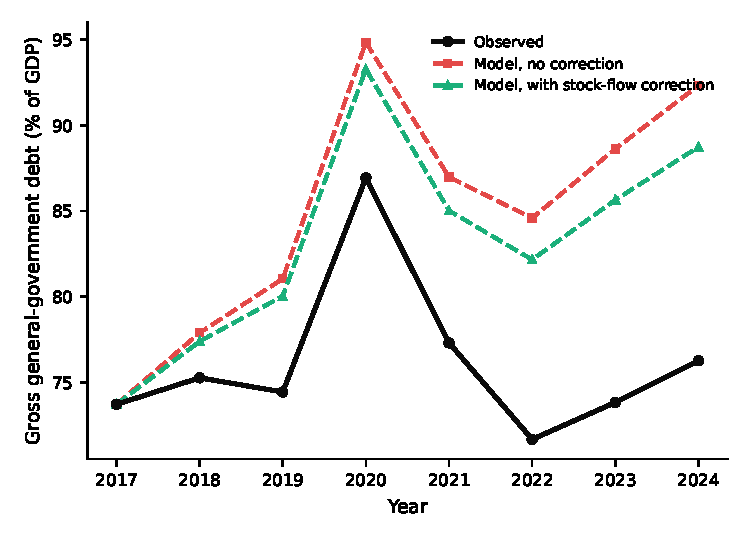
\includegraphics[width=0.85\textwidth]{figures/backtest_fit.pdf}
\caption{Tier 2: observed Brazilian gross general-government debt/GDP, 2017--2024, against the model's own debt-identity recursion anchored once in 2017, with and without the 2011--2017 mean stock-flow-adjustment correction. Neither reconstruction recovers the observed post-2021 decline; both overshoot by 2024 (16.1~pp and 12.5~pp of GDP respectively).}
\label{fig:backtest-fit}
\end{figure}

We consider this an important result in its own right, not merely a caveat. The residual is not evenly distributed: the single largest contributor is a set of discretionary Treasury-to-BNDES lending and BNDES early-repayment and Central Bank result-transfer operations between 2011 and 2022, which move the implied stock-flow adjustment by as much as 3.9~pp of GDP in a single year and show no relationship to any macroeconomic covariate --- growth, interest rates, the terms of trade or the sovereign spread --- available to the model. These are discretionary policy decisions, not quantities any forward-looking macro model, however well specified, could have predicted several years in advance, a description that fits squarely within the broader literature on quasi-fiscal operations of public financial institutions \citep{mackenziestella1996} and on stock-flow adjustments as a large, persistent and only partly explicable source of debt accumulation worldwide \citep{weber2012sfa,seiferling2013}: \citet{jaramilloetal2017}'s finding, from 179 historical debt-spike episodes, that spikes driven by stock-flow adjustments rather than primary deficits predict debt subsequently \emph{failing} to decline, is a genuinely sobering precedent for how Brazil's own episode should be read (the fuller positioning of this literature, including the closest peer-reviewed treatment of the Brazilian episode specifically, is in the online supplementary material's literature review). Rather than search for a better-fitting correction, which would mean fitting noise, we instead represent this uncertainty honestly: a stochastic stock-flow-adjustment term, bootstrapped in three-year blocks from the demeaned 2011--2024 historical series and applied identically to every scenario within a Monte Carlo draw (so that it widens absolute debt-level uncertainty without mechanically favouring any policy), is added to the published Monte Carlo as of the most recent run. This does not and cannot make the point-forecast back-test pass; it instead ensures that published debt-level \emph{ranges}, where they are shown at all, are not falsely narrow. We regard the choice between a better point estimate and an honestly wider interval, when the former is simply unavailable, as itself a methodological contribution worth stating plainly: a model that cannot forecast a quantity should say so by widening its uncertainty, not by implicitly asserting precision it does not have.

A further internal review identified that the growth-block Tier~1 check had originally reused a fixed total-factor-productivity growth rate estimated over 2000--2019, a window that fully contains the 2006--2019 test period, so that its pass demonstrated internal consistency rather than held-out predictive skill, unlike the debt-identity check (a pure accounting relationship with no fitted parameter) and the external-channel check (fitted on 2000--2014, tested on 2015--2024 only). This has since been corrected: the growth-block statistic is now estimated on a genuinely pre-sample total-factor-productivity window (1996--2005, ending seven years before the test period begins) and the Tier~1 gate is re-keyed to this corrected statistic, which the model passes more comfortably than the original, contaminated one (mean absolute error $-0.036$ against $0.165$~pp of GDP a year). We report the original defect, and its fix, explicitly, because it is precisely the kind of in-sample contamination that a less self-critical validation exercise would allow to pass unremarked, and because a corrected statistic that happens to pass more easily than the flawed one it replaces is itself worth distinguishing from a corrected statistic that was simply re-engineered until it passed.

\subsection{Diagnostic extensions: a brief summary}
\label{sec:d4}

Tier~2's failure leaves open a question the back-test itself cannot answer: how much of the headline status-quo debt path is an artefact of the model's deliberately simple, no-policy-reaction specification, and how much would a more behaviourally realistic government, or a more aggressively nonlinear market response, change it? The online supplementary material reports, in full, a set of clearly labelled, off-by-default diagnostics built to answer exactly this, run only against the status-quo baseline (\textsc{S0}) and never folded into any published Monte Carlo summary. In brief: under the model's own preferred specification, including the stochastic stock-flow-adjustment term of Section~\ref{sec:backtest}, the probability that \textsc{S0}'s debt ratio exceeds 90\% of GDP is already 73.6\% at five years and 95.0\% by ten; a fiscal-reaction-function variant using Brazil's own, counter-intuitively signed estimated coefficient produces a \emph{higher}, not lower, debt path than the unconditional baseline; and an explicitly nonlinear, fiscal-fatigue-style risk-premium variant, following \citet{ghoshkimmendozaostryqureshi2013} and \citet{bi2012}, stays close to the model's existing linear premium below a historical threshold but diverges sharply above it. Every absolute figure in that supplementary material inherits the same Tier~2 bias documented above and should be read accordingly, as an upper-bound diagnostic rather than a calibrated forecast.

A different, equally natural question is not whether the status-quo debt path is realistic, but whether the paired scenario \emph{differences} of Table~\ref{tab:headline} themselves are biased by channels the model omits (the business cycle, a monetary reaction function, the exchange rate and the distribution of interest income). The online supplementary material reports six further off-by-default diagnostics built as a direct sanity check on exactly this, and Section~\ref{sec:discussion} gives the resulting answer in full.

% ===========================================================================
\section{Headline results}
\label{sec:results}
% ===========================================================================

We report here only indicators that have cleared the Tier~1 gate, as paired differences against the status-quo baseline; absolute debt levels are reported as differences versus \textsc{S0}, never as validated levels, consistent with Section~\ref{sec:backtest}. Readers wanting the fuller, Tier-2-honest picture of \textsc{S0}'s own absolute debt level --- breach probabilities, the fiscal gap, and the fiscal-reaction-function and nonlinear-premium diagnostics --- should turn to the online supplementary material, which is deliberately not folded into the paired-difference table below. All figures are the median across one thousand draws, with the 10th--90th percentile range in brackets, for the default package composition and the transitory-multiplier persistence setting unless stated otherwise.

\begin{figure}[htbp]
\centering
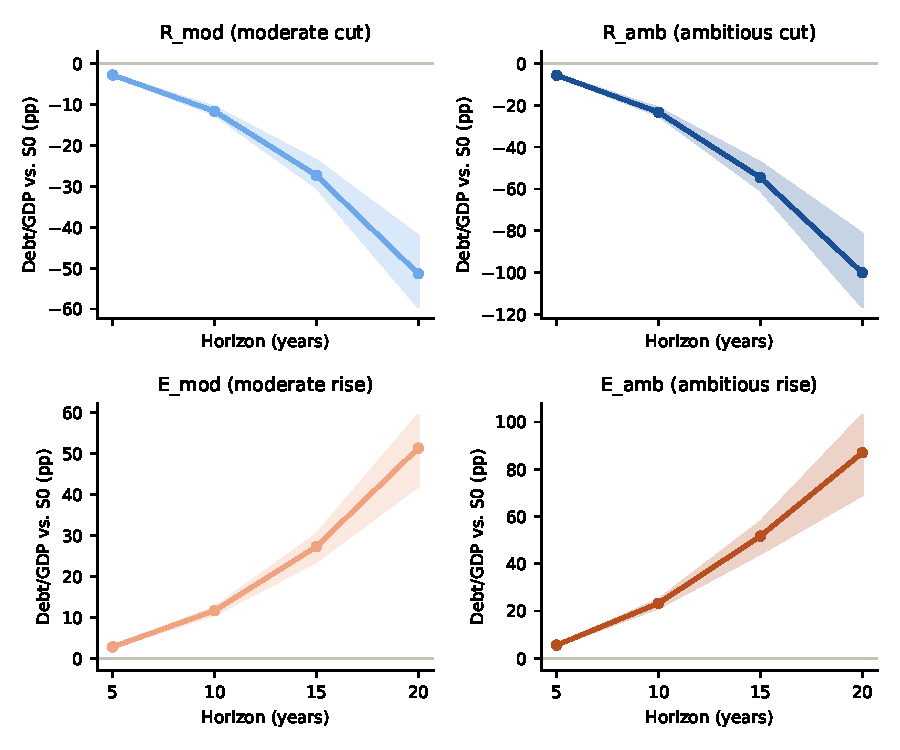
\includegraphics[width=\textwidth]{figures/debt_fan.pdf}
\caption{Debt/GDP vs.\ \textsc{S0}, by scenario and horizon: median (line) and parameter-uncertainty band (shaded, 10th--90th percentile) across one thousand draws, default composition, transitory multiplier persistence. Reported only at the model's four named horizons (5/10/15/20 years), joined for legibility, not a continuous forecast path --- the bands describe resampled parameter uncertainty, not a conditional quantile forecast (Section~\ref{sec:montecarlo}).}
\label{fig:debt-fan}
\end{figure}

\begin{figure}[htbp]
\centering
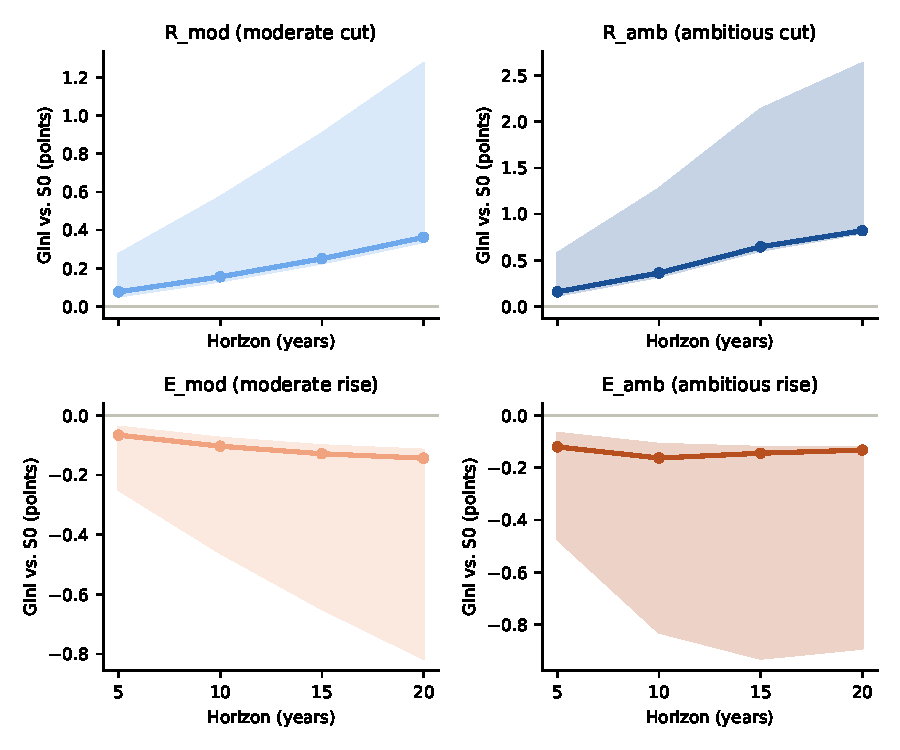
\includegraphics[width=\textwidth]{figures/gini_fan.pdf}
\caption{Gini coefficient vs.\ \textsc{S0}, by scenario and horizon, same data and convention as Figure~\ref{fig:debt-fan}.}
\label{fig:gini-fan}
\end{figure}

\begin{table}[htbp]
\centering
\small
\caption{Selected ten-year (2035) scenario effects against the status-quo baseline, default composition, transitory multiplier persistence. Median [p10, p90] across 1,000 Monte Carlo draws.}
\label{tab:headline}
\resizebox{\textwidth}{!}{%
\begin{tabular}{lrrrr}
\toprule
Indicator & \textsc{R\_mod} (moderate cut) & \textsc{R\_amb} (ambitious cut) & \textsc{E\_mod} (moderate rise) & \textsc{E\_amb} (ambitious rise) \\
\midrule
GDP level vs.\ S0 (\%) & $-0.40$ $[-0.48,-0.31]$ & $-0.79$ $[-0.97,-0.62]$ & $+0.40$ $[+0.31,+0.48]$ & $+0.79$ $[+0.62,+0.97]$ \\
Debt/GDP vs.\ S0 (pp) & $-11.6$ $[-12.4,-10.7]$ & $-23.3$ $[-24.7,-21.4]$ & $+11.6$ $[+10.7,+12.4]$ & $+23.3$ $[+21.4,+24.7]$ \\
Unemployment vs.\ S0 (pp) & $+0.07$ $[+0.06,+0.09]$ & $+0.14$ $[+0.11,+0.17]$ & $-0.07$ $[-0.09,-0.06]$ & $-0.14$ $[-0.17,-0.11]$ \\
Infant mortality vs.\ S0 (per 1,000) & $+0.035$ $[+0.017,+0.055]$ & $+0.069$ $[+0.034,+0.110]$ & $-0.035$ $[-0.056,-0.017]$ & $-0.070$ $[-0.112,-0.035]$ \\
Gini vs.\ S0 (points) & $+0.16$ $[+0.13,+0.57]$ & $+0.36$ $[+0.33,+1.27]$ & $-0.10$ $[-0.46,-0.08]$ & $-0.16$ $[-0.83,-0.11]$ \\
\bottomrule
\end{tabular}%
}
\end{table}

Three features of these results are worth drawing out, visible directly in Figures~\ref{fig:debt-fan} and~\ref{fig:gini-fan} as well as in Table~\ref{tab:headline}. First, the central ten-year reduction in debt from an ambitious, sustained 4~pp-of-GDP consolidation is a little under 24~pp of GDP against the status-quo baseline, roughly in line with the arithmetic of the debt identity rather than requiring any output-side heroics; Figure~\ref{fig:debt-fan} shows every scenario's p10--p90 band widening by a strikingly consistent factor of roughly ten between the ten- and twenty-year horizons (9.9--10.3$\times$ across all four scenarios), so parameter-uncertainty growth here tracks horizon rather than policy ambition. The GDP cost of achieving the consolidation is under one percentage point at the median under transitory multipliers, but rises to a median GDP loss of 3.9\% at ten years under the persistent-multiplier assumption (Section~\ref{sec:architecture}), a difference large enough that no single headline number for ``the cost of consolidation'' is defensible without stating which multiplier persistence assumption it uses. Second, the status-quo debt path itself, with no policy change, rises from 78.6\% to a central 145.5\% of GDP by 2035, of which 61\% of the ten-year increase is attributable to the interest-growth differential rather than to the (ageing-driven) widening of the primary deficit; this is the arithmetic fact that gives any debt-stabilisation rule, of the kind proposed in the challenger's 2026 programme, its force, independently of whether the specific numerical target chosen is the right one. Third, every reduction scenario raises the simulated Gini coefficient and infant mortality, and every expansion scenario lowers both, by magnitudes consistent in direction, if not in exact size, with the cross-country consolidation literature \citep{ballfurcerilleighlloungani2013} and the Brazilian health-spending elasticity literature \citep{szkloclarkerocha2024} on which the two blocks separately draw --- a consistency we read as mildly reassuring given that neither block was calibrated to reproduce the other's finding. Figure~\ref{fig:gini-fan} shows this holds up under the model's own parameter uncertainty, not only at the median: none of the four scenarios' p10--p90 Gini bands cross zero at any reported horizon, so the sign of the headline Gini effect is robust to the sampled parameters this Monte Carlo varies. The reversal discussed in Section~\ref{sec:discussion} comes from a channel this Monte Carlo does not sample at all --- interest income's incidence, added only in the online supplementary material --- not from parameter uncertainty within the published run.

For a reader who wants the policy-relevant content of this paper without the two 2026 programmes' withheld headline comparison, these three findings are it: the composition and persistence of any fiscal adjustment matter at least as much as its headline size; the interest-growth differential, not discretionary policy, is the arithmetic force driving status-quo debt upward, which is what gives a debt-stabilisation rule of the kind either candidate might adopt its logic independently of the specific target chosen; and any reduction large enough to bend the debt path materially also moves distributional and health outcomes in the same direction, by an amount this paper reports rather than assumes away.

% ===========================================================================
\section{Discussion: what this model is, and is not, for}
\label{sec:discussion}
% ===========================================================================

Three limitations deserve emphasis beyond those already noted in the discussion of each block.

\emph{This is a comparative-statics and accounting instrument, not a dynamic stochastic general-equilibrium model, and the omitted channels plausibly, though not demonstrably, bias the expansion scenarios' reported distributional improvement.} Prices, wages and behaviour do not adjust endogenously to a change in fiscal policy except through the specific, named channels described above (a fiscal multiplier, an Okun-law unemployment response, a household's mechanical exposure to a given tax or transfer change). There is no labour-supply response, no portfolio reallocation, no monetary-policy reaction function, and no general-equilibrium price adjustment. This is a deliberate choice: each of those omitted channels is itself contested in the literature, and we judged it more honest to omit a channel entirely, and say so, than to include a stylised version calibrated to no particular Brazilian estimate. But the omission is not symmetric in its likely consequence, and a direct sanity check on the model's own completeness makes exactly this point: a sustained, debt-financed expansion would plausibly trigger a connected chain this model does not price at any link --- a higher policy rate as the Central Bank responds to the resulting inflation and debt trajectory, a weaker real as fiscal stress widens the sovereign spread, higher borrowing costs crowding out private investment, an inflation tax that falls hardest on poor households' largely non-indexed cash holdings, and higher interest payments accruing disproportionately to the bondholders who are concentrated in the top income centiles. Every one of these channels runs in the direction of raising, not lowering, the measured Gini and poverty cost of an expansion, which is why the model's own finding that expansions mechanically lower the Gini coefficient (Section~\ref{sec:results}) should be read as the effect of the transfer and tax channels \emph{alone}, holding monetary policy, the currency and private portfolio income fixed, not as a net welfare statement. Unlike the general-equilibrium channels we have not attempted to quantify, two of these specific channels --- interest income distributed the way it is actually concentrated, and a Taylor-rule Selic response to a scenario's own output gap --- are quantified in full as off-by-default diagnostics in the online supplementary material, run separately from, and never folded into, Table~\ref{tab:headline}. The answer is not a hedge: combining each diagnostic's own median effect with the published figure (in that supplementary material's synthesis discussion) moves \textsc{E\_mod}'s and \textsc{E\_amb}'s median ten-year Gini effect from $-0.10$ and $-0.16$ points to $+0.65$ and $+1.15$ points respectively --- the distributional finding \emph{reverses sign} once interest income is distributed correctly, and the debt cost of both scenarios is understated by roughly 13--14\%. We regard this as settling the direction of this hypothesis, for the specific channels we could quantify, while still not settling the channels we could not (the labour-supply and portfolio-reallocation responses named above remain genuinely unquantified).

\emph{Public debt is modelled as a single undifferentiated stock, with no split by indexation, currency or holder, though the composition this omits is, for Brazil specifically, concentrated in a domestic-rate risk the model already prices rather than a currency risk it does not.} The debt-accumulation identity (Section~\ref{sec:architecture}) applies one interest rate to the entire debt stock; it does not distinguish Selic-linked floating-rate bonds from inflation-linked, fixed-rate or foreign-currency-linked instruments, and the exchange rate (Section~\ref{sec:architecture}) affects debt only through inflation pass-through, never through direct revaluation of foreign-currency liabilities. This is a genuine simplification, but its practical consequence for Brazil is smaller than for a dollar-indebted emerging market: on the Brazilian National Treasury's own most recent published composition, Selic-linked (floating-rate) instruments are both the largest share of federal domestic debt and a rapidly rising one (48.3\% at the close of 2025, 52.7\% by August 2026, against a revised 2026 target band of 49--53\%), inflation-linked instruments a further fifth to a quarter, fixed-rate instruments a fifth, and foreign-exchange-linked instruments a stable 3.7--4.4\% of the total, a range the Treasury's own borrowing plan keeps essentially unchanged year on year \citep{tesourormd2026}. Separately, roughly 96\% of federal debt is placed in the domestic market \citep{tesourormd2026}. The composition risk this model therefore omits is overwhelmingly the one it already prices through the debt identity's single interest rate and the sovereign-risk-premium channel, namely a rise in the Selic (the Treasury's own published sensitivity: a 1~pp rise in the Selic adds approximately R\$60.6~billion, about 0.46\% of GDP, to gross debt in year one alone, \citealp{tesourormd2026}), not the foreign-currency revaluation risk a multi-currency debt model would be built to capture. We quantify this valuation adjustment directly in the online supplementary material: it is indeed small at this paper's main ten-year horizon, confirming the framing above, but grows to a median 5--17~pp of GDP by twenty years under the common bootstrapped exchange-rate path, and remains small (under 0.5~pp at twenty years) even once the depreciation itself is made to respond to a scenario's own fiscal stress rather than drawn unconditionally --- confirming that this channel stays small because the underlying FX-linked share is small, not because the mechanism linking fiscal stress to the exchange rate is inert.

\emph{The model cannot and does not attempt to assess the corruption propensity, competence, or governing quality of any candidate or government.} Both the routine-leakage parameter and the major-corruption shock process are, by explicit design, applied identically to every scenario and to both 2026 programmes within a Monte Carlo draw; this is not a simplifying assumption adopted for convenience, but a direct consequence of the fact that the only available perception-based measures of Brazilian governance quality --- the World Bank's Control of Corruption estimate and the Transparency International Corruption Perceptions Index --- cannot, within their own stated measurement uncertainty, distinguish recent Brazilian administrations from one another. A model that tried to assign different corruption parameters to different candidates on the basis of these indices would be manufacturing precision the underlying data does not support.

\emph{The model's single most consequential finding may be about its own limits rather than about fiscal policy.} The Tier~2 back-test failure documented in Section~\ref{sec:backtest} is a substantive result: a model built from a textbook debt-accumulation identity, careful growth accounting, and an explicitly estimated external-sector channel still cannot reproduce six years of observed Brazilian debt accumulation to within five percentage points of GDP, because a material part of that accumulation is driven by discretionary balance-sheet operations between the Treasury, the development bank BNDES and the Central Bank that have no macroeconomic antecedent a model of this kind could observe in advance. This is not a peculiarly Brazilian failing: the wider stock-flow-adjustment literature surveyed in the online supplementary material finds the same pattern --- large, persistent, poorly-explained residuals --- across more than a hundred countries \citep{weber2012sfa}, and finds that large residuals of exactly this kind predict debt subsequently failing to decline \citep{jaramilloetal2017}, which is precisely why we chose to widen the model's uncertainty bands rather than search for a better-fitting correction. Any debt-sustainability exercise for Brazil --- ours or another's --- that reports a single confident debt-level projection without confronting this fact should, we think, be read with considerable scepticism.

\emph{The Monte Carlo reports a resampled distribution, not a true conditional quantile forecast, and the distributional block omits a fiscal-impoverishment measure.} The percentiles reported throughout this paper, including the breach probabilities reported in the online supplementary material, describe the spread induced by resampling independently drawn structural parameters; they are not the output of a quantile regression conditioned on the current state of the economy, in the sense the growth-at-risk and debt-at-risk literature now uses the term \citep{prasadetal2019growthatrisk,lianpresbiterowiriadinata2020,furcerietal2025debtrisk}. Extending the model to condition its percentiles on observable pre-shock conditions, rather than treating every draw as exchangeable, is a natural next step we have not undertaken. Separately, the household microsimulation reports the Gini coefficient and two poverty headcounts but not the fiscal-impoverishment measure of \citet{higginslustig2016}, which would show directly whether any household is left poorer in absolute terms by a package that is, on the Gini and headcount measures reported here, both progressive and poverty-reducing; closing this gap would strengthen the distributional claims made in Section~\ref{sec:results} without requiring any new data source.

% ===========================================================================
\section{Conclusion}
\label{sec:conclusion}
% ===========================================================================

We have described a modular, stochastic framework for evaluating changes in the size and composition of the Brazilian state, chaining a demographic fiscal baseline, a growth-and-debt macro block, a household microsimulation, a social-outcomes block, a set of long-run feedback channels, an external-sector block, and an explicit governance layer, propagated through a thousand-draw Monte Carlo and checked, as far as the available data permit, against Brazil's own fiscal history. Applied to a common grid of reduction and expansion scenarios, the model finds that the composition and persistence assumptions attached to a given fiscal adjustment matter at least as much as its headline size; that population ageing alone will raise age-related spending by several percentage points of GDP over the coming decade regardless of policy; that the interest-growth differential, not the primary balance, is projected to be the dominant driver of status-quo debt accumulation; and that the model's own historical back-test, read honestly, fails to validate any single confident debt-level projection, a failure we trace to discretionary balance-sheet operations no macro-fiscal model of this design could have anticipated, and which an independently documented, cross-country stock-flow-adjustment literature suggests is a structural feature of sovereign debt accounting rather than a peculiarly Brazilian one. In direct response to that failure, we report --- as a clearly labelled, off-by-default diagnostic never folded into the headline results --- how much the status-quo debt path would change under a typical emerging-market fiscal-reaction coefficient, under Brazil's own, oppositely-signed estimated coefficient, and under an explicitly nonlinear, fiscal-fatigue-style risk premium, together with EC/IFI-style breach probabilities and a fiscal-gap statement that a bare median debt path cannot provide. Applied, as a methodological demonstration, to the two candidate programmes filed for Brazil's 2026 presidential run-off, the same machinery shows that a constitutional spending-growth rule and an explicit debt-stabilising rule are, formally, two different closure rules for the same debt-accumulation identity, whose consequences depend on assumptions --- about composition, about delivery against stated targets, about privatisation proceeds --- that neither candidate's own published programme fully specifies; we withhold the resulting headline comparison from this paper pending the same internal validation gate applied to every other result. We offer the framework itself, and the discipline of its parameter registry and its publication gate, as the paper's principal contribution: a fiscal scenario model is, in our view, more useful for the questions it refuses to answer with false precision than for the ones it answers confidently.

Read only as an accounting exercise, not a recommendation, four things the model's own numbers imply are worth weighing in the next term. The interest-growth differential, not spending size, drives most of the status-quo debt increase (Section~\ref{sec:results}), so credibility that compresses the sovereign-risk premium would plausibly do more than any single consolidation's headline size \citep{blanchard2019,furmansummers2020}. The model's own package-composition sensitivities, consistent with the wider composition-of-consolidation literature \citep{alesinaardagna2010,pires2014}, suggest protecting public investment and administrative efficiency ahead of pension indexation would moderate any adjustment's growth and distributional cost. Ring-fencing health spending has a quantified, not merely plausible, payoff for child mortality \citep{szkloclarkerocha2024,rasellaetal2013}. And a debt-financed expansion's distributional benefit is not automatic: the online supplementary material shows it depends on whether the resulting interest income is left with its actual, concentrated holders \citep{lustig2018ceq,higginspereira2014} or paired with an instrument that claws some of it back. None of this ranks the two 2026 programmes (Section~\ref{sec:scenarios}) or forecasts what either would do; it is what this paper's own quantified trade-offs imply, stated with the same hedges attached to every other number in this paper.

% ===========================================================================
\section*{Data and code availability}
% ===========================================================================
\addcontentsline{toc}{section}{Data and code availability}
The code, configuration, and the complete parameter registry required to reproduce every result in this paper, together with a README describing how each table and figure is generated, are openly available in the public GitHub repository \url{https://github.com/AugustoFM/minimal-state-world-dashboard}, hosted under the author's own personal account (the handle ``AugustoFM'' combines his middle and first names with his surname initial, in that order). A permanent tag or release pinned to the exact commit underlying this submitted version will be created at the time of submission and referenced here, so that reproduction of the results in Table~\ref{tab:headline} and the online supplementary material's tables does not depend on the repository's actively developed main branch. The repository includes: the full simulation codebase (data preparation, macro, microsimulation, social, feedback, external and Monte Carlo modules); the single machine-readable parameter registry recording, for every numerical input used in any published result, its source, vintage, licence and a verification flag; the task-by-task development log (\texttt{tasks/STATUS.md}) documenting each modelling decision and its review; and the scripts that generate Table~\ref{tab:headline} and the online supplementary material's tables directly from the committed Monte Carlo output. Raw PNAD Cont\'inua microdata are not redistributed in the repository, in line with IBGE's own distribution terms, but are freely downloadable from IBGE and the repository's data-preparation scripts reconstruct the exact extract used here from that public source. No other dataset used in this paper is proprietary or restricted.

% ===========================================================================
\section*{Funding}
% ===========================================================================
\addcontentsline{toc}{section}{Funding}
This research received no specific grant from any funding agency in the public, commercial, or not-for-profit sectors. The author is an independent researcher and undertook this work without institutional affiliation or external funding.

% ===========================================================================
\section*{Conflict of interest}
% ===========================================================================
\addcontentsline{toc}{section}{Conflict of interest}
The author declares no conflict of interest. The author has no financial, professional or personal relationship with either candidate or campaign referenced in Section~\ref{sec:scenarios}, and the programme-mapping exercise described there is explicitly withheld from headline publication pending the model's own internal validation gate, a decision made for methodological rather than political reasons.

% ===========================================================================
\section*{Ethics statement}
% ===========================================================================
\addcontentsline{toc}{section}{Ethics statement}
This study uses only secondary, publicly available official statistics and anonymised government survey microdata (IBGE's PNAD Cont\'inua); it involves no original data collection from human participants, no identifiable personal data, and no intervention. No ethics committee approval was required or sought.

% ===========================================================================
\section*{Author contributions}
% ===========================================================================
\addcontentsline{toc}{section}{Author contributions}
Flaviano A.\ Moreira: Conceptualisation; Methodology; Software; Validation; Formal analysis; Investigation; Data curation; Writing -- original draft; Writing -- review and editing; Visualisation; Project administration. (CRediT taxonomy; sole author.)

% ===========================================================================
\section*{Acknowledgements and disclosure of AI-assisted tools}
% ===========================================================================
\addcontentsline{toc}{section}{Acknowledgements and disclosure of AI-assisted tools}
In accordance with the publisher's policy on generative artificial intelligence, the author discloses the following uses of AI technologies in producing this paper and the research underlying it. \emph{Research methodology, software development and data analysis:} the simulation codebase (approximately fifteen thousand lines across the data-preparation, macro, microsimulation, social, feedback, external and Monte Carlo modules) was developed iteratively with the assistance of AI coding agents, principally Anthropic's Claude Code (Claude Opus and Sonnet model families, 2026) and OpenAI's Codex (GPT-5-series models, 2026), operating throughout under the author's direct and continuous direction. The author specified every modelling choice and equation, reviewed and tested all AI-generated code, and is solely responsible for the model's design, its validation (Section~\ref{sec:backtest}), and its limitations. \emph{Literature review:} the extended literature review in the online supplementary material was compiled with the assistance of AI research agents that conducted targeted web searches to locate and verify candidate citations; every citation retained in this paper was independently checked by the author against a publicly accessible primary or indexing source (the publisher's own page, NBER, IMF, RePEc/IDEAS, or an equivalent repository) before inclusion, and candidate citations that could not be so verified were excluded rather than retained on the strength of the AI agent's own assertion. \emph{Manuscript drafting and editing:} AI language-model assistance (the same Claude model family) was used in drafting and iteratively revising the prose of this manuscript under the author's direction; the author reviewed, edited and takes full responsibility for the final text, its arguments, and its conclusions. No AI tool is credited as an author, consistent with the principle that authorship requires the capacity to take responsibility for the work, which these tools do not have. Every numerical parameter used in any published result is independently recorded, with its source, vintage, licence and a verification flag, in the machine-readable registry described in the Data and Code Availability statement above; parameters without a traceable source are marked explicitly as such and excluded from headline results. The author thanks no individual funder or institution, consistent with the Funding statement above.

% ===========================================================================
\bibliographystyle{plainnat}
\begin{thebibliography}{73}
\bibitem[Acemoglu and Johnson, 2007]{acemoglujohnson2007} Acemoglu, D. and Johnson, S. (2007). Disease and Development: The Effect of Life Expectancy on Economic Growth. \textit{Journal of Political Economy}, 115(6), 925--985.

\bibitem[Akerman et al., 2025]{akermanetal2025} Akerman, A., Moscona, J., Pellegrina, H.S.\ and Sastry, K.\ (2025). Public R\&D Meets Economic Development: Embrapa and Brazil's Agricultural Revolution. \textit{NBER Working Paper} No.\ 34213.

\bibitem[Alcantara and Kannebley Jr., 2024]{alcantarakannebley2024} Alcantara, R.C.\ de\ and Kannebley Jr., S.\ (2024). Elasticidade de P\&D na ind\'ustria brasileira e transbordamentos: uma abordagem de fatores comuns n\~ao observados. \textit{Economia Aplicada}, 28(1), 89--127.

\bibitem[Alesina and Ardagna, 2010]{alesinaardagna2010} Alesina, A. and Ardagna, S. (2010). Large Changes in Fiscal Policy: Taxes versus Spending. \textit{Tax Policy and the Economy}, 24(1), 35--68.

\bibitem[Alesina et al., 2015]{alesinafaverogiavazzi2015} Alesina, A., Favero, C. and Giavazzi, F. (2015). The Output Effect of Fiscal Consolidation Plans. \textit{Journal of International Economics}, 96(S1), S19--S42.

\bibitem[Andrews, 2023]{andrews2023} Andrews, M.J.\ (2023). How Do Institutions of Higher Education Affect Local Invention? Evidence from the Establishment of U.S.\ Colleges. \textit{American Economic Journal: Economic Policy}, 15(2), 1--41.

\bibitem[Auerbach and Gorodnichenko, 2012]{auerbachgorodnichenko2012} Auerbach, A.J.\ and Gorodnichenko, Y.\ (2012). Measuring the Output Responses to Fiscal Policy. \textit{American Economic Journal: Economic Policy}, 4(2), 1--27.

\bibitem[Avis, Ferraz and Finan, 2018]{avisferrazfinan2018} Avis, E., Ferraz, C. and Finan, F. (2018). Do Government Audits Reduce Corruption? Estimating the Impacts of Exposing Corrupt Politicians. \textit{Journal of Political Economy}, 126(5), 1912--1964.

\bibitem[Baldacci and Kumar, 2010]{baldaccikumar2010} Baldacci, E. and Kumar, M.S. (2010). Fiscal Deficits, Public Debt, and Sovereign Bond Yields. \textit{IMF Working Paper} WP/10/184.

\bibitem[Balladares and Garc\'ia-Miralles, 2026]{balladaresgarciamiralles2026} Balladares, S.\ and Garc\'ia-Miralles, E.\ (2026). Fiscal Drag with Microsimulation: Evidence from Spanish Tax Records. \textit{Fiscal Studies}, Early View.

\bibitem[Ball et al., 2013]{ballfurcerilleighlloungani2013} Ball, L., Furceri, D., Leigh, D. and Loungani, P. (2013). The Distributional Effects of Fiscal Consolidation. \textit{IMF Working Paper} WP/13/151.

\bibitem[Banco Central do Brasil]{bcbsgs} Banco Central do Brasil. Sistema Gerenciador de S\'eries Temporais (SGS): general-government gross debt series 13762, Selic and IPCA series. \url{https://www3.bcb.gov.br/sgspub}.

\bibitem[Bi, 2012]{bi2012} Bi, H.\ (2012). Sovereign Default Risk Premia, Fiscal Limits and Fiscal Policy. \textit{European Economic Review}, 56(3), 389--410.

\bibitem[Blanchard, 2019]{blanchard2019} Blanchard, O.\ (2019). Public Debt and Low Interest Rates. \textit{American Economic Review}, 109(4), 1197--1229.

\bibitem[Bloom, Canning and Sevilla, 2001]{bloomcanningsevilla2001} Bloom, D.E., Canning, D. and Sevilla, J. (2001). The Effect of Health on Economic Growth: Theory and Evidence. \textit{NBER Working Paper} No.\ 8587.

\bibitem[Bom and Ligthart, 2014]{bomligthart2014} Bom, P.R.D.\ and Ligthart, J.E. (2014). What Have We Learned from Three Decades of Research on the Productivity of Public Capital? \textit{Journal of Economic Surveys}, 28(5), 889--916.

\bibitem[Bourguignon and Spadaro, 2006]{bourguignonspadaro2006} Bourguignon, F.\ and Spadaro, A.\ (2006). Microsimulation as a Tool for Evaluating Redistribution Policies. \textit{Journal of Economic Inequality}, 4(1), 77--106.

\bibitem[Celasun, Debrun and Ostry, 2007]{celasundebrunostry2007} Celasun, O., Debrun, X.\ and Ostry, J.D.\ (2007). Primary Surplus Behavior and Risks to Fiscal Sustainability in Emerging Market Countries: A ``Fan-Chart'' Approach. \textit{IMF Staff Papers}, 53(3), 401--425.

\bibitem[Cordes et al., 2015]{cordesetal2015} Cordes, T., Kinda, T., Muthoora, P.\ and Weber, A.\ (2015). Expenditure Rules: Effective Tools for Sound Fiscal Policy? \textit{IMF Working Paper} WP/15/29.

\bibitem[\'Egert, 2015]{egert2015} \'Egert, B.\ (2015). Public Debt, Economic Growth and Nonlinear Effects: Myth or Reality? \textit{Journal of Macroeconomics}, 43, 226--238.

\bibitem[Feenstra, Inklaar and Timmer, 2015]{pwt1001} Feenstra, R.C., Inklaar, R.\ and Timmer, M.P.\ (2015). The Next Generation of the Penn World Table. \textit{American Economic Review}, 105(10), 3150--3182. (Series version 10.01, Groningen Growth and Development Centre.)

\bibitem[Feenstra et al., Human Capital in PWT]{pwt1001human} Feenstra, R.C., Inklaar, R.\ and Timmer, M.P.\ Human Capital in PWT Version 9.0, PWT documentation note.

\bibitem[Feld and Kirchg\"assner, 2008]{feldkirchgassner2008} Feld, L.P.\ and Kirchg\"assner, G.\ (2008). On the Effectiveness of Debt Brakes: The Swiss Experience. \textit{CREMA Working Paper}.

\bibitem[Ferraz, Finan and Moreira, 2012]{ferrazfinanmoreira2012} Ferraz, C., Finan, F.\ and Moreira, D.B.\ (2012). Corrupting Learning: Evidence from Missing Federal Education Funds in Brazil. \textit{Journal of Public Economics}, 96(9--10), 712--726.

\bibitem[Filmer and Pritchett, 1999]{filmerpritchett1999} Filmer, D.\ and Pritchett, L.\ (1999). The Impact of Public Spending on Health: Does Money Matter? \textit{Social Science \& Medicine}, 49(10), 1309--1323.

\bibitem[Furceri et al., 2025]{furcerietal2025debtrisk} Furceri, D., Giannone, D., Kisat, F., Lam, W.R.\ and Li, H.\ (2025). Debt-at-Risk. \textit{IMF Working Paper} 25/086.

\bibitem[Furman and Summers, 2020]{furmansummers2020} Furman, J.\ and Summers, L.H.\ (2020). A Reconsideration of Fiscal Policy in the Era of Low Interest Rates. Discussion draft, Brookings Hutchins Center / Peterson Institute for International Economics.

\bibitem[Gallet and Doucouliagos, 2017]{gallet2017} Gallet, C.A.\ and Doucouliagos, H.\ (2017). The Impact of Healthcare Spending on Health Outcomes: A Meta-Regression Analysis. \textit{Social Science \& Medicine}, 179, 9--17.

\bibitem[Garcia and Rigobon, 2004]{garciarigobon2004} Garcia, M.\ and Rigobon, R.\ (2004). A Risk Management Approach to Emerging Market's Sovereign Debt Sustainability with an Application to Brazilian Data. \textit{NBER Working Paper} No.\ 10336.

\bibitem[Ghosh et al., 2013]{ghoshkimmendozaostryqureshi2013} Ghosh, A.R., Kim, J.I., Mendoza, E.G., Ostry, J.D.\ and Qureshi, M.S.\ (2013). Fiscal Fatigue, Fiscal Space and Debt Sustainability in Advanced Economies. \textit{Economic Journal}, 123(566), F4--F30.

\bibitem[Gobetti and Orair, 2017]{gobettiorair2017} Gobetti, S.W.\ and Orair, R.O.\ (2017). Contas P\'ublicas Acima da Linha. \textit{IPEA Texto para Discuss\~ao} No.\ 2288.

\bibitem[Gruss, 2014]{gruss2014} Gruss, B.\ (2014). After the Boom--Commodity Prices and Economic Growth in Latin America and the Caribbean. \textit{IMF Working Paper} WP/14/154.

\bibitem[Guajardo, Leigh and Pescatori, 2014]{guajardoleighpescatori2014} Guajardo, J., Leigh, D.\ and Pescatori, A.\ (2014). Expansionary Austerity? International Evidence. \textit{Journal of the European Economic Association}, 12(4), 949--968.

\bibitem[Hanousek and Ko\v{c}enda, 2011]{hanousekkocenda2011} Hanousek, J.\ and Ko\v{c}enda, E.\ (2011). Public Investment and Fiscal Performance in the New EU Member States. \textit{Fiscal Studies}, 32(1), 43--71.

\bibitem[Herndon, Ash and Pollin, 2014]{herndonashpollin2014} Herndon, T., Ash, M.\ and Pollin, R.\ (2014). Does High Public Debt Consistently Stifle Economic Growth? A Critique of Reinhart and Rogoff. \textit{Cambridge Journal of Economics}, 38(2), 257--279.

\bibitem[Higgins and Lustig, 2016]{higginslustig2016} Higgins, S.\ and Lustig, N.\ (2016). Can a Poverty-Reducing and Progressive Tax and Transfer System Hurt the Poor? \textit{Journal of Development Economics}, 122, 63--75.

\bibitem[Higgins and Pereira, 2014]{higginspereira2014} Higgins, S.\ and Pereira, C.\ (2014). The Effects of Brazil's Taxation and Social Spending on the Distribution of Household Income. \textit{Public Finance Review}, 42(3), 346--367.

\bibitem[IBGE, 2024]{ibge2024} Instituto Brasileiro de Geografia e Estat\'istica (2024). Proje\c{c}\~ao da Popula\c{c}\~ao do Brasil, revis\~ao 2024.

\bibitem[Instituição Fiscal Independente, 2021]{ifi2021ee16} Instituição Fiscal Independente (2021). Estudo Especial n.\textsuperscript{o} 16: Elasticidade de longo prazo da receita federal.

\bibitem[Instituição Fiscal Independente, 2023]{ifi2023raf76} Instituição Fiscal Independente, Senado Federal (2023). Relat\'orio de Acompanhamento Fiscal No.\ 76 (maio de 2023).

\bibitem[IMF, 2026]{imfweo2026} International Monetary Fund (2026). World Economic Outlook database, Brazil country series.

\bibitem[Ilzetzki, Mendoza and V\'egh, 2013]{ilzetzkimendozavegh2013} Ilzetzki, E., Mendoza, E.G.\ and V\'egh, C.A.\ (2013). How Big (Small?) Are Fiscal Multipliers? \textit{Journal of Monetary Economics}, 60(2), 239--254.

\bibitem[Jaramillo, Mulas-Granados and Kimani, 2017]{jaramilloetal2017} Jaramillo, L., Mulas-Granados, C.\ and Kimani, E.\ (2017). Debt Spikes and Stock-Flow Adjustments: Emerging Economies in Perspective. \textit{Journal of Economics and Business}, 94, 1--14.

\bibitem[Jones and Williams, 1998]{joneswilliams1998} Jones, C.I.\ and Williams, J.C.\ (1998). Measuring the Social Return to R\&D. \textit{Quarterly Journal of Economics}, 113(4), 1119--1135.

\bibitem[Karam and Hostland, 2005]{karamhostland2005} Karam, P.D.\ and Hostland, D.\ (2005). Assessing Debt Sustainability in Emerging Market Economies Using Stochastic Simulation Methods. \textit{IMF Working Paper} 05/226.

\bibitem[Karam and Hostland, 2006]{karamhostland2006} Karam, P.D.\ and Hostland, D.\ (2006). Specification of a Stochastic Simulation Model for Assessing Debt Sustainability in Emerging Market Economies. \textit{IMF Working Paper} 06/268.

\bibitem[Kopits and Symansky, 1998]{kopitssymansky1998} Kopits, G.\ and Symansky, S.\ (1998). Fiscal Policy Rules. \textit{IMF Occasional Paper} No.\ 162.

\bibitem[Lago-Pe\~nas, Cadaval-Sampedro and Herrero-Alcalde, 2024]{lagopenasetal2024} Lago-Pe\~nas, S., Cadaval-Sampedro, M.\ and Herrero-Alcalde, A.\ (2024). Fiscal Consolidation and Voting: On the Electoral Costs of Budgetary Stability. \textit{Fiscal Studies}, 45(4), 559--581.

\bibitem[Levy Yeyati and Sturzenegger, 2023]{levyyeyatisturzenegger2023} Levy Yeyati, E.\ and Sturzenegger, F.\ (2023). A Balance-Sheet Approach to Fiscal Sustainability. \textit{Fiscal Studies}, 44(1), 61--84.

\bibitem[Lian, Presbitero and Wiriadinata, 2020]{lianpresbiterowiriadinata2020} Lian, W., Presbitero, A.F.\ and Wiriadinata, U.\ (2020). Public Debt and r-g at Risk. \textit{IMF Working Paper} 20/137.

\bibitem[Litschig, 2012]{litschig2012} Litschig, S.\ (2012). Are Rules-Based Government Programs Shielded from Special-Interest Politics? Evidence from Revenue-Sharing Transfers in Brazil. \textit{Journal of Public Economics}, 96(11--12), 1047--1060.

\bibitem[Litschig and Morrison, 2013]{litschig2013} Litschig, S.\ and Morrison, K.M.\ (2013). The Impact of Intergovernmental Transfers on Education Outcomes and Poverty Reduction. \textit{American Economic Journal: Applied Economics}, 5(4), 206--240.

\bibitem[L\'opez-Villavicencio and Zoumenou, 2025]{lopezvillavicencio2025} L\'opez-Villavicencio, A.\ and Zoumenou, D.W.\ (2025). Deficit Bias and the Effectiveness of EU Fiscal Rules. \textit{Journal of Macroeconomics}, 84.

\bibitem[Lustig, 2018]{lustig2018ceq} Lustig, N.\ (ed.) (2018). \textit{Commitment to Equity Handbook: Estimating the Impact of Fiscal Policy on Inequality and Poverty}. Brookings Institution Press / CEQ Institute, Tulane University.

\bibitem[Mackenzie and Stella, 1996]{mackenziestella1996} Mackenzie, G.A.\ and Stella, P.\ (1996). Quasi-Fiscal Operations of Public Financial Institutions. \textit{IMF Occasional Paper} No.\ 142.

\bibitem[Mauro, 1995]{mauro1995} Mauro, P.\ (1995). Corruption and Growth. \textit{Quarterly Journal of Economics}, 110(3), 681--712.

\bibitem[National Transfer Accounts, Brazil]{nta2018} National Transfer Accounts project. Brazil age-profile accounts, vintages 2003 and 2018.

\bibitem[Nunes et al., 2020]{nunesetal2020} Nunes, A.\ et al.\ (2020). O Impacto do Resultado do Banco Central do Brasil para o Cumprimento da Regra de Ouro. \textit{Desenvolvimento em Quest\~ao}, Unijuí.

\bibitem[Olken, 2007]{olken2007} Olken, B.A.\ (2007). Monitoring Corruption: Evidence from a Field Experiment in Indonesia. \textit{Journal of Political Economy}, 115(2), 200--249.

\bibitem[Ostry, Berg and Tsangarides, 2014]{ostrybergtsangarides2014} Ostry, J.D., Berg, A.\ and Tsangarides, C.G.\ (2014). Redistribution, Inequality, and Growth. \textit{IMF Staff Discussion Note} SDN/14/02.

\bibitem[Panizza and Presbitero, 2014]{panizzapresbitero2014} Panizza, U.\ and Presbitero, A.F.\ (2014). Public Debt and Economic Growth: Is There a Causal Effect? \textit{Journal of Macroeconomics}, 41, 21--41.

\bibitem[Pires, 2014]{pires2014} Pires, M.C.C.\ (2014). Pol\'itica Fiscal e Ciclos Econ\^omicos no Brasil. \textit{Economia Aplicada}, 18(1), 69--90.

\bibitem[Pires, 2019]{pires2019reggraouro} Pires, M.\ (2019). Uma An\'alise da Regra de Ouro no Brasil. \textit{Revista de Economia Pol\'itica}, 39(1).

\bibitem[Prasad et al., 2019]{prasadetal2019growthatrisk} Prasad, A., Elekdag, S., Jeasakul, P., Lafarguette, R., Alter, A., Feng, A.X.\ and Wang, C.\ (2019). Growth at Risk: Concept and Application in IMF Country Surveillance. \textit{IMF Working Paper} 19/036.

\bibitem[Ramey and Zubairy, 2018]{rameyzubairy2018} Ramey, V.A.\ and Zubairy, S.\ (2018). Government Spending Multipliers in Good Times and in Bad: Evidence from US Historical Data. \textit{Journal of Political Economy}, 126(2), 850--901.

\bibitem[Rasella et al., 2013]{rasellaetal2013} Rasella, D., Aquino, R., Santos, C.A.T., Paes-Sousa, R.\ and Barreto, M.L.\ (2013). Effect of a Conditional Cash Transfer Programme on Childhood Mortality: A Nationwide Analysis of Brazilian Municipalities. \textit{The Lancet}, 382(9886), 57--64.

\bibitem[Reinhart and Rogoff, 2010]{reinhartrogoff2010} Reinhart, C.M.\ and Rogoff, K.S.\ (2010). Growth in a Time of Debt. \textit{American Economic Review}, 100(2), 573--578.

\bibitem[Resende and Pires, 2021]{resendepires2021} Resende, C.T.\ and Pires, M.\ (2021). O Impulso de Multiplicador Fiscal: Implementa\c{c}\~ao e Evid\^encia para o Brasil. \textit{Estudos Econ\^omicos}, 51(2), 213--243.

\bibitem[Sanches, 2026]{sanches2026} Sanches, M.\ et al.\ (2026). Adjustment Through Revenue or Spending? Fiscal Adjustment Scenarios Based on Estimated Multiplier Effects. \textit{Estudos Econ\^omicos}, 56.

\bibitem[Secretaria do Tesouro Nacional, 2025]{tesouro2025} Secretaria do Tesouro Nacional (2025). Estat\'isticas Fiscais do Governo Geral (GFSM 2014), 2025-IV.

\bibitem[Secretaria do Tesouro Nacional, COFOG, 2024]{tesourocofog2024} Secretaria do Tesouro Nacional (2024). Classifica\c{c}\~ao Funcional (COFOG) do Governo Geral, 2024.

\bibitem[Secretaria do Tesouro Nacional, RMD, 2026]{tesourormd2026} Secretaria do Tesouro Nacional (2026). Relat\'orio Mensal da D\'ivida (RMD), composi\c{c}\~ao por indexador (dezembro de 2025 e agosto de 2026) e Plano Anual de Financiamento (PAF) 2026, faixas revisadas em 26 de agosto de 2026; Selic sensitivity (R\$60.6 billion per 1pp) and domestic-market debt share as reported in Secretaria do Tesouro Nacional press releases reproduced by Ag\^encia Gov and Ag\^encia Brasil, \url{https://agenciagov.ebc.com.br} and \url{https://agenciabrasil.ebc.com.br}, accessed 2026-10-26.

\bibitem[Seiferling, 2013]{seiferling2013} Seiferling, M.\ (2013). Stock-Flow Adjustments, Government's Integrated Balance Sheet, and Fiscal Transparency. \textit{IMF Working Paper} 2013/063.

\bibitem[Szklo, Clarke and Rocha, 2024]{szkloclarkerocha2024} Szklo, A., Clarke, D.\ and Rocha, R.\ (2024). Public Health Spending and Infant Mortality: Evidence from Brazil. \textit{IZA Discussion Paper} No.\ 16829.

\bibitem[IBGE, PNAD Cont\'inua, 2025]{pnad2025} Instituto Brasileiro de Geografia e Estat\'istica (2025). Pesquisa Nacional por Amostra de Domic\'ilios Cont\'inua, primeira visita.

\bibitem[Valero and Van Reenen, 2019]{valerovanreenen2019} Valero, A.\ and Van Reenen, J.\ (2019). The Economic Impact of Universities: Evidence from Across the Globe. \textit{Economics of Education Review}, 68, 53--67.

\bibitem[Weber, 2012]{weber2012sfa} Weber, A.\ (2012). Stock-Flow Adjustments and Fiscal Transparency: A Cross-Country Comparison. \textit{IMF Working Paper} WP/12/39.

\bibitem[Woo, Bova, Kinda and Zhang, 2017]{woobovakindazhang2017} Woo, J., Bova, E., Kinda, T.\ and Zhang, Y.S.\ (2017). Distributional Consequences of Fiscal Adjustments: What Do the Data Say? \textit{IMF Economic Review}, 65(2), 273--307.

\end{thebibliography}

\end{document}
